The contrast between finite-difference and finite-element approximation is 
greatest in that finite-difference works in terms of sample points on a regular
grid as indicated in \Sec{geomprob},
whereas finite-element uses an approximation for the solutions interior
to arbitrarily shaped ``elements".
The resulting systems of equations for the discretised fields, eg.\
meaning the finite-difference mesh values
$f_j, j=1,\ldots,N$, also tend to lend themselves to very different methods of
solution. Indeed for simple explicit finite-difference schemes the very concept of 
solving a matrix equation is not required, being replaced by simple
updates in place. This approach tends to be inefficient in finite-elements because
the elements have different sizes, and as remarked in \Sec{geomprob}
the maximum stepsize is restricted by the smallest cells, leading to
implicit schemes that require solution of large systems of linear
equations (sparse matrix equations) for finite element nodal values~$f_j$.

%\clearpage
\subsection{Spectral/hp Elements}\label{sec:semsub}
One justification for use of the term~`spectral' in this context is that early
experiments were made with Fourier series approximations within
the elements. Thus when difficulties were encountered with this
`spectrally accurate' approach and polynomials replaced the trigonometric
functions, the terminology `spectral' was retained to emphasise that high order
polynomials could achieve the same level of theoretical accuracy.

The~$hp$ in the name simply indicates by the~$h$ that finite elements of
very different spatial sizes are allowed and by the~$p$ that arbitrarily
large polynomial orders~$p$ may be exploited. Spectral accuracy may
conceived of as the limiting result $p\rightarrow\infty$, although
in practice the order~$p$ seldom exceeds~$10$.

\begin{figure}[h]
\centerline{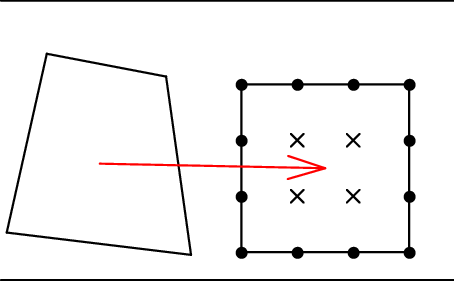
\includegraphics[width=6cm]{../pics/mapquad}
\hspace{1cm}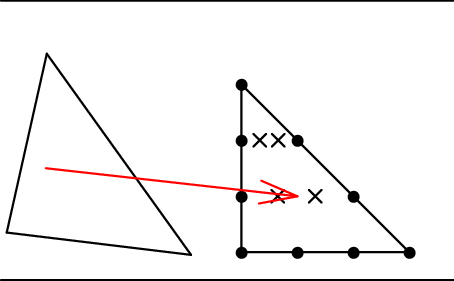
\includegraphics[width=6cm]{../pics/maptri}}
\centerline{(a) \hspace{7cm} (b)}
\caption{An arbitrary planar quadrilateral is mapped to the
unit square (a) and a triangle to a reference triangle (b).
\label{fig:maps}}
\end{figure}

Since the publication of the book by Karniadakis and Sherwin, %\cite{karniadakissherwin}
spectral/hp element has tended to taken on a more specific meaning, namely the use
of Lagrangian interpolation polynomials with nodes at certain specific
`Gauss' points in the elements. Each coordinate direction is treated
separately in this way, and different shaped elements are mapped to
squares or cubes of unit sidelength in order for it to work, see \Fig{maps}.
A key point
is that the mapping between `reference space' and real space can be singular
without disaster for the overall algorithm, thus elements
which are triangles and prisms in real space may be accommodated,
see \Fig{maps}(b).

\begin{figure}[h]
\centerline{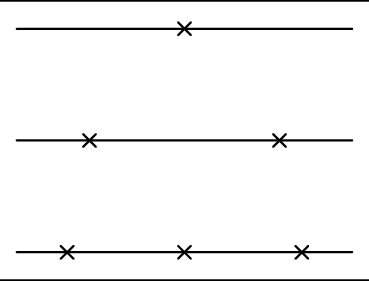
\includegraphics[width=6cm]{../pics/gauxpts}
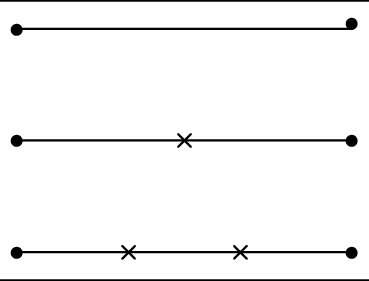
\includegraphics[width=6cm]{../pics/gaulob} }
\centerline{(a) \hspace{7cm} (b)}
\caption{(a) left, intervals marked with Gauss points~$x_{Gj}$
for integrations using respectively from top to bottom, totals of $1$, $2$ and~$3$ samples.
(b) right, are indicated the Gauss-Lobatto points 
for integrations using respectively from top to bottom, totals of $2$, $3$ and~$4$ samples.
\label{fig:gausspts}}
\end{figure}

Gauss points answer the question about the least number of samples
needed to integrate a polynomial of given order over an interval, by giving the
locations of the sample points, and corresponding weights. If only 
one sample point is used, then this should obviously be at the centre
of the interval, but if two are used, it turns out they should be
located at $x=\pm G_1 = \pm 0.577\,350$ when the interval is $-1 \leq x \leq 1$,
and similarly for three points $x=0$, $x=\pm G_2 = \pm 0.774\,597$,
see \Fig{gausspts}(a).
As an aside, this last example implies for the mapped spectral/hp element, three basis functions
which as Lagrangian interpolants are respectively proportional to
\begin{equation} \label{eq:lagpoly}
(x+G_2)x,\;\; x(x-G_2),\;\mbox{and}\; (x+G_2)(x-G_2)
\end{equation}
The general Gauss quadrature formula for integrating a polynomial is
\begin{equation} \label{eq:gaussint}
\int_{-1}^{+1} p(x) dx = \sum_{j=1}^{n} w_{Gj} p(x_{Gj}) 
\end{equation}
where $p(x)$ is the polynomial, $x_{Gj},j=1,\ldots n$ are Gauss points and
$w_{Gj}$ are the corresponding weights, which are tabulated in
numerical analysis texts such as Stoer and Bulirsch. %\cite[\S\,3.6]{stoerbulirsch}
Since the latter points and weights
represent $2n$~degrees of freedom, it turns out that polynomials of order
up to~$2n-1$ can always be integrated exactly in this manner.

However, the better finite element approximations seemingly always
involve placing nodes at element edges, so it becomes necessary to work
with the so-called Gauss-Lobatto points that give maximum accuracy when two of
the $x_{Gj}$ are forced to lie at the interval ends~$x=\pm 1$,
see \Fig{gausspts}(b).  These points
are tabulated by Boyd. %\cite[Appendix F10]{boyd}

\clearpage
\subsection{Working with Spectral/hp Elements}\label{sec:semwork}
Establishing the convergence properties of finite element methods generally requires use of
much heavier mathematics than finite-difference, so this section only touches on key
issues. The most basic operation for discretising partial differential equations
is forming the partial derivative~$\partial f/\partial x$.

Suppose that spectral/hp
elements provide a basis~$\chi_j$, so that a field~$f(x)$ may be represented
\begin{equation}
f(x) = \sum_j f_j \chi_j(x)
\end{equation}
and its derivative has coefficients $f'_j$, then 
\begin{equation}
 \frac{\partial f}{\partial x}= \sum_j f'_j \chi_j(x) \approx \sum_j f_j \frac{\partial \chi_j}{\partial x}
\end{equation}
If $\chi_j(x)$ is a polynomial, then clearly the two discrete expressions
cannot be equal pointwise, but they can be equated in the weak sense.
This is to be interpreted as meaning that the two must have the same
inner product with every member of the basis~$\chi_i, i=1,\ldots N$
\begin{eqnarray}\label{eq:weakdx}
\sum_j f'_j \langle \chi_j, \chi_i \rangle & = & \sum_j f_j \langle \frac{\partial \chi_j}{\partial x}, \chi_i \rangle, \;\; \mbox{ each } i\\
\mbox{where the mass matrix } M_{ij}=\langle \chi_j, \chi_i \rangle & = &  \int_{a}^{b} \chi_j(x) \chi_i(x) dx
\label{eq:inprod}
\end{eqnarray}
Now the significance of interpolation at the Gauss points becomes apparent
since by construction each Lagrange interpolant~$\chi_j$  vanishes at all but one
of these points, which not only reduces
the number of arithmetic operations required to evaluate the mass matrix,
but means that Gauss point interpolation also \emph{diagonalises} the matrix.
%is diagonal, requiring no special inversion techniques.

\clearpage
\subsection{Galerkin versus Discontinuous Galerkin with Spectral/hp Elements}\label{sec:gvsdg}

\begin{figure}
\centerline{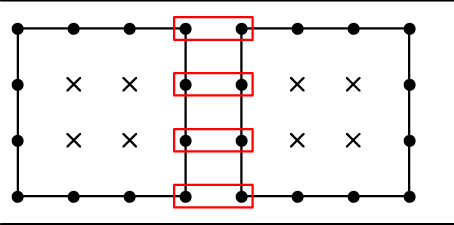
\includegraphics[width=12cm]{../pics/gaulob2d}}
\caption{This shows the locations of Gauss-Lobatto points
on two adjacent reference squares, with the positions of edge nodes
marked using circles, and interior nodes as crosses. In the
usual Galerkin formulation the edge nodes within each red box
have a shared value, whereas in Discontinuous Galerkin these values
are allowed to differ, even though they represent the same point.
\label{fig:gaulob2d}}
\end{figure}
The description of the preceding \Sec{semwork} regarding the
mass matrix has been a little misleading, since
with regular Gauss points, the nodes within each element are effectively decoupled
from those in all other elements, so a practical calculation of $f'_j$
accounting for boundary conditions would not be possible.
%so a realistic calculation would  soon take values
%that almost certainly diverged from one element to another.
Within the standard spectral/hp element
usage of Gauss-Lobatto points, the edge nodes have a special status. The classical
Galerkin formulation implies that the edge nodal value is shared between
at least two elements (more at corners of 2-D elements etc.), see \Fig{gaulob2d},
which has the
effect of coupling this pair of elements together and hence ultimately every node of
every element. (In practice to save storage, the shared nodal value
is saved only once.) However, there is another
option for a surprisingly wide class of problems, which is to allow different
values at these edge nodes in the different elements, even though they correspond
to the same point in space. Typically the (nodal values on different) elements 
are then linked only by means of a flux
condition, giving the Discontinuous Galerkin~(DG) method, so-called for
the obvious reason. 

It is worth commenting on the complementarity of  the finite-element approach relative to finite-difference,
for even though spectral/hp element gives at best  a continuous approximation
to~$f(x)$ at inter-element boundaries, the order of convergence measured in the
energy norm will be of high polynomial order~$p$ in the space variable. 
Crudely speaking, for finite-element, large errors at isolated points are swamped by the accurate integrals
taken over the rest of the interval (and analogously in higher dimensions). Compare
finite-differences, where high order is only enforced at isolated grid-points.

In contrast to other finite-element polynomial bases, transient calculations
with spectral elements do not necessarily require a matrix inversion. However,
integrals such as the right-hand-side of \Eq{weakdx} do couple different elements and thus to
avoid timestep restrictions on a mesh with a wide range of sizes,
will have to be treated at least partly implicitly.
However, the spectral element formulation is here such that if the edge nodal values are known
then the values at the internal modes may be constructed from them. Thus the matrix
equation for implicit time advance that includes the discrete~$\partial /\partial x$ operator,
need only be solved for the edge nodes, at a massive reduction in cost for
high order elements, as highlighted by
Karniadakis and Sherwin.  %\cite[\S\,4.2.3]{karniadakissherwin}
It was not initially realised that the just-described `static condensation' approach to
inverting spectral element matrices could also be extended to Discontinuous
Galerkin, and the ultimate realisation led to the Hybridisable Discontinuous
Galerkin or HDG~algorithm. 

It emerges that HDG and Galerkin methods may be competitive in many problems
involving fluxes. The discontinuity in HDG makes for robustness in 
situations where the physics may support discontinuous solutions,
eg.\ when solving transport equations with practically no dissipation.
On the other hand the discontinuity comes at considerable cost in storage
for there is not just duplication at edge nodes, but the replacement of
one value needed in the Galerkin formulation
by $8$~field values at say, the corners of hexahedral elements.
For practical values of~$p$, the storage overhead of HDG is at least~$50$\,\%,
although this can often be offset by exceptionally large rates of
convergence (`superconvergence') at special nodes.

%Studies indicate that the balance between HDG and Galerkin
%is so fine in classical hydrodynamics
%that it is down to how the (reduced size) matrix problem is solved,
%specifically the selection of preconditioner. %\cite{Ya16ToCG}.






